%% This is file `DEMO-TUDaPub.tex' version 2.09 (2020/03/13),
%% it is part of
%% TUDa-CI -- Corporate Design for TU Darmstadt
%% ----------------------------------------------------------------------------
%%
%%  Copyright (C) 2018--2020 by Marei Peischl <marei@peitex.de>
%%
%% ============================================================================
%% This work may be distributed and/or modified under the
%% conditions of the LaTeX Project Public License, either version 1.3c
%% of this license or (at your option) any later version.
%% The latest version of this license is in
%% http://www.latex-project.org/lppl.txt
%% and version 1.3c or later is part of all distributions of LaTeX
%% version 2008/05/04 or later.
%%
%% This work has the LPPL maintenance status `maintained'.
%%
%% The Current Maintainers of this work are
%%   Marei Peischl <tuda-ci@peitex.de>
%%   Markus Lazanowski <latex@ce.tu-darmstadt.de>
%%
%% The development respository can be found at
%% https://github.com/tudace/tuda_latex_templates
%% Please use the issue tracker for feedback!
%%
%% ============================================================================
%%
% !TeX program = lualatex
%%

\documentclass[
	ngerman,
	accentcolor=1c,% Farbe für Hervorhebungen auf Basis der Deklarationen in den Corporate Design Richtlinien
%	logofile=example-image, %Falls die Logo Dateien nicht vorliegen
	]{tudapub}

\usepackage[english, main=ngerman]{babel}
\usepackage[babel]{csquotes}

\usepackage{biblatex}
\bibliography{DEMO-TUDaBibliography}

%Formatierungen für Beispiele in diesem Dokument. Im Allgemeinen nicht notwendig!
\let\file\texttt
\let\code\texttt
\let\pck\textsf
\let\cls\textsf

\usepackage{hologo}




\begin{document}

%Zusätzliche Metadaten für PDF/A. In diesem Fall notwendig, weil Titel ein Makro enthält.
\Metadata{
	author=NeXT,
	title=Space Workshop Rating,
	%subject=Basisdokumentation und Template zur Nutzung der tudapub-Dokumentenkasse,
	%date=2019-04-29,
	%keywords=TU Darmstadt \sep Corporate Design \sep LaTeX
}




\title{Workshop\newline Vorbereitung}
\subtitle{NeXT Generation on Campus}
%\author{Marei Peischl\thanks{pei\TeX{} \TeX{}nical Solutions}\and der \TeX-Löwe}
\date{}
%\titleimage{
%%	%Folgende Box kann selbstverständlich durch ein mit \includegraphics geladenes Bild ersetzt werden.
%\bigskip
%\bigskip
%\bigskip
%\bigskip
%\bigskip
%\bigskip
%\bigskip
%\bigskip
%\bigskip
%\bigskip
%\bigskip
%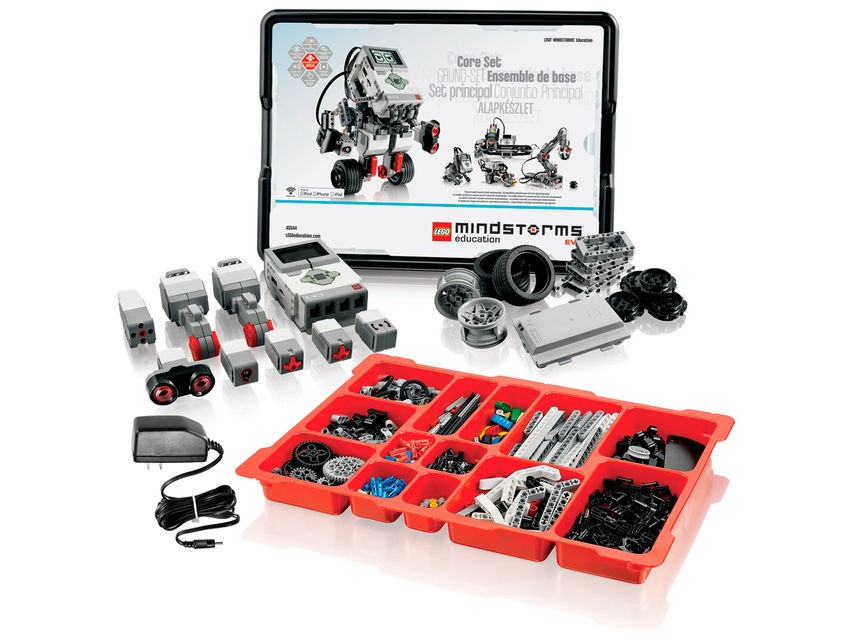
\includegraphics[width=\textwidth]{../control/images/title.jpg}
%	%\color{black!30}\rule{\width}{\height}
%}


%Varianten der Infoboxen
\addTitleBox{\includegraphics[width=\linewidth]{../../ist_logo.pdf}}
%\addTitleBoxLogo{example-image}
%\addTitleBoxLogo*{\includegraphics[width=.3\linewidth]{example-image}}



\maketitle


\newpage


\tableofcontents
\section{Einf\"uhrung}
In diesem Dokument werden einige Hinweise bereitgestellt, die vor und zu Beginn des Workhops hilfreich sind.

\section{Vorbereitung}
In diesem Abschnitt werden die einzelnen Schritte vor dem Workshop gelistet und es werden kurze Hinweise gegeben um Unklarheiten und h\"aufige Probleme bei der Durchf\"uhrung zu vermeiden.

\subsection{Space}
Vor dem Workshop m\"ussen die Spielpl\"ane aufgebaut werden, auf dem Plan und auf den Stationen sind jeweils Klettverschl\"usse angebracht, sodass man dadurch besser erkennen kann, welche Station an welcher Stelle platziert werden muss. Ebenso gibt es auf der Lego-Seite hilfreiche Bilder zum Aufbau. Beim Anbringen ist darauf zu achten, dass die Stationen mit Druck fest und stabil angebracht werden. \newline
F\"ur einen fairen Wettkampf ist es ebenso wichtig, dass die beiden Spielpl\"ane identisch aufgebaut werden, das gilt besonders f\"ur die gleiche Reihenfolge des Weltraumschrotts und der Astronauten. Ebenso muss die Satellitensch\"ussel an der vorderen Position eingehakt werden, damit sie sich sp\"ater richtig aufstellt.\\
F\"ur die Bearbeitung muss an jedem PC ein Baukasten, ein EV3-Brick sowie eine Anleitung und pro Team ein Wertungsbogen vorhanden sein.

\subsection{MindroidLejos}
F\"ur die Bearbeitung muss an jedem PC ein Baukasten, ein EV3-Brick sowie eine Anleitung vorhanden sein.\\
Falls zuletzt die Mindroid-Variante durchgef\"uhrt wurde, muss auf dem Brick zun\"achst die PAN-Einstellung ge\"andert werden. Hierbei muss der AP-Modus gew\"ahlt werden und die IP 10.0.0.1 gespeichert werden.

\subsection{Mindroid}
F\"ur den Mindroid-Workshop wird pro PC ein Roboter (oder zwei f\"ur die Kommunikation) und die Aufgabenstellung und Anleitung ben\"otigt. Ebenso muss der Router angeschaltet werden.\\
Falls zuletzt die MindroidLejos-Variante durchgef\"uhrt wurde, muss auf dem Brick zun\"achst die PAN-Einstellung ge\"andert werden. Hierbei muss der USB-Modus gew\"ahlt werden und die IP 192.168.0.42 gespeichert werden.

\section{Durchf\"uhrung}
In diesem Abschnitt werden Hinweise besonders f\"ur den Beginn der Veranstaltung gegeben.

\subsection{Space}
Zu Beginn des Workshops ist es wichtig, den genauen Ablauf des Wettkampfs durchzugehen inklusive der Erl\"auterung der einzelnen Stationen da hier oft Unklarheiten entstehen.\newline
Auch hat es sich bew\"ahrt einen klaren Zeitplan vorzugeben und nach einer Einarbeitungszeit ein Teammeeting anzusetzen, so ergibt sich ein gutes, motiviertes Arbeitsklima.\newline
Je nach Leistungsstand der Gruppe ist es sehr sinnvoll, gemeinsam ein kurzes Programm zu schreiben und zu testen.
\\Zum Ende ist es besonders wichtig auch Zeit zum Aufr\"aumen einzuplanen. In den Sortierk\"asten befinden sich Bilder sodass die Sch\"uler die Teile wieder einordnen k\"onnen und man am Schluss auf Vollst\"andigkeit \"uberpr\"ufen kann, das ist besonders bei den elektronischen Bauteilen wichtig.

\subsection{Mindroid}
Ein h\"aufig auftretendes Problem ist die lockere Verbindung zwischen den Komponenten, daher ist es hilfreich, dass die Sch\"uler zu Beginn alle Kabel \"uberpr\"ufen, ob sie sicher eingesteckt sind.\newline
Da die \"Ubertragung auf das Handy oft beim ersten Mal Schwierigkeiten bereitet, ist es sehr zu empfehlen, zu Beginn gemeinsam ein Programm zu starten.\\


\subsection{MindroidLejos}
Ein h\"aufig auftretendes Problem ist die lockere Verbindung zwischen den Komponenten, daher ist es hilfreich, dass die Sch\"uler zu Beginn alle Kabel \"uberpr\"ufen, ob sie sicher eingesteckt sind.\newline




\cfoot{\textcolor{lightgray} \today}




\end{document}
